\section{Eseguire il progetto base}

\subsection{Algoritmo}

La base dell'algoritmo permette all'utente di scegliere un raggio massimo per il cluster. 

Per ciascun punto interessato, ossia i punti con distanza inferiore al raggio impostato, l'algoritmo calcola i cluster candidati.

Una volta individuati i cluster, quello con il numero maggiore di punti verrà salvato nella cartella \texttt{./results/}, ossia nella root del progetto base. Il nome del file indicherà il database di partenza e il raggio massimo utilizzato per la ricerca, quindi scegliendo per esempio il database \texttt{gopicnic} con un raggio di 3, il file di output sarà \texttt{gopicnic\_003.dmp}.

\begin{figure}[h!]
    \centering
    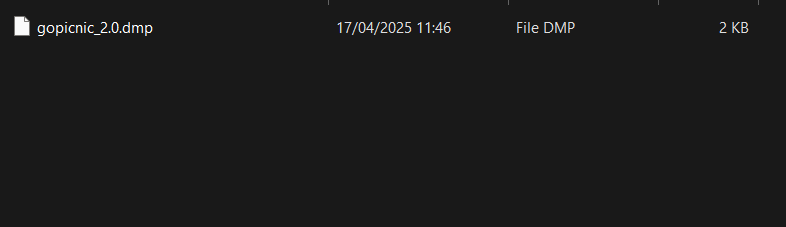
\includegraphics[width = 0.5 \textwidth]{images/results.png}
    \caption{Risultati del salvataggio}
    
\end{figure}

Una volta creato il file di output, l'algoritmo provvederà ad eliminare anche i cluster non salvati, per evitare che vengano esaminati nuovamente. 

Nel caso in cui più di un cluster abbia il numero massimo di punti, l'algoritmo ripeterà la procedura con il set ridotto di punti. 

\subsection{Struttura del progetto base}

Il progetto base consiste in un'applicazione di tipo client/server. Di fatto, nella cartella \texttt{Jar+Bat} sono presenti i file \texttt{start\_server.bat} per l'esecuzione del server e \texttt{start\_client} per il client, che non sono altro che degli script batch per l'esecuzione dei file jar.

\begin{figure}[h!]
    \centering
    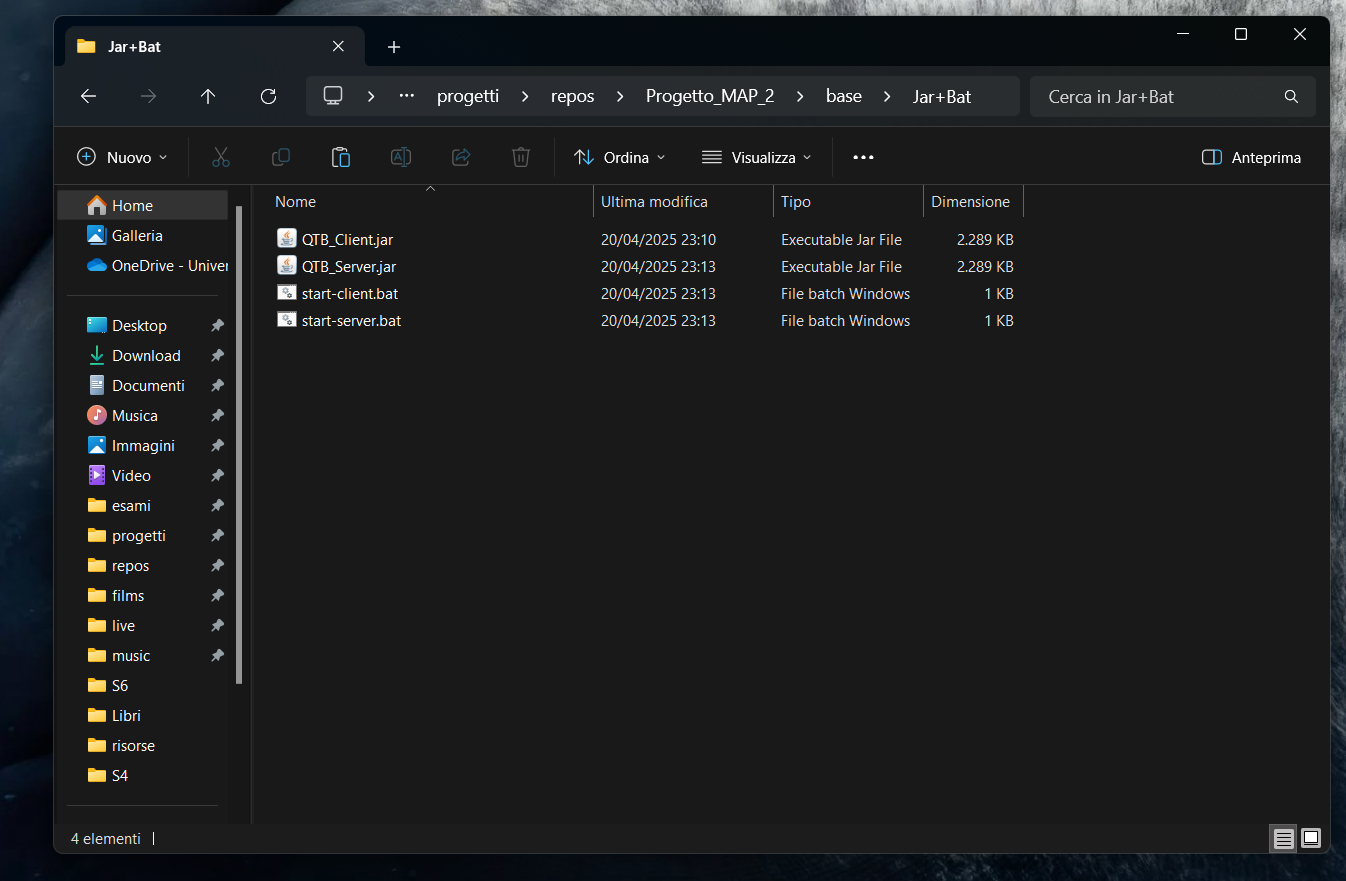
\includegraphics[width = 0.5 \textwidth]{images/file jar base.png}
    \caption{Jar del progetto base}
\end{figure}


\begin{tcolorbox}[  colback=white!5!white, colframe=gray, title={Avvertenza} ]

    Per avviare il programma correttamente, è necessario eseguire prima il file \texttt{.bat} del server e poi quello del client.
\end{tcolorbox}

\subsection{Esecuzione di QTB\_Server}


Il normale avviamento del file \texttt{start\_server.bat} mostrerà la seguente schermata, che indica che il server è in ascolto sulla porta 8080, in attesa di una richiesta da parte del client.

\begin{figure}[h!]
    \centering
    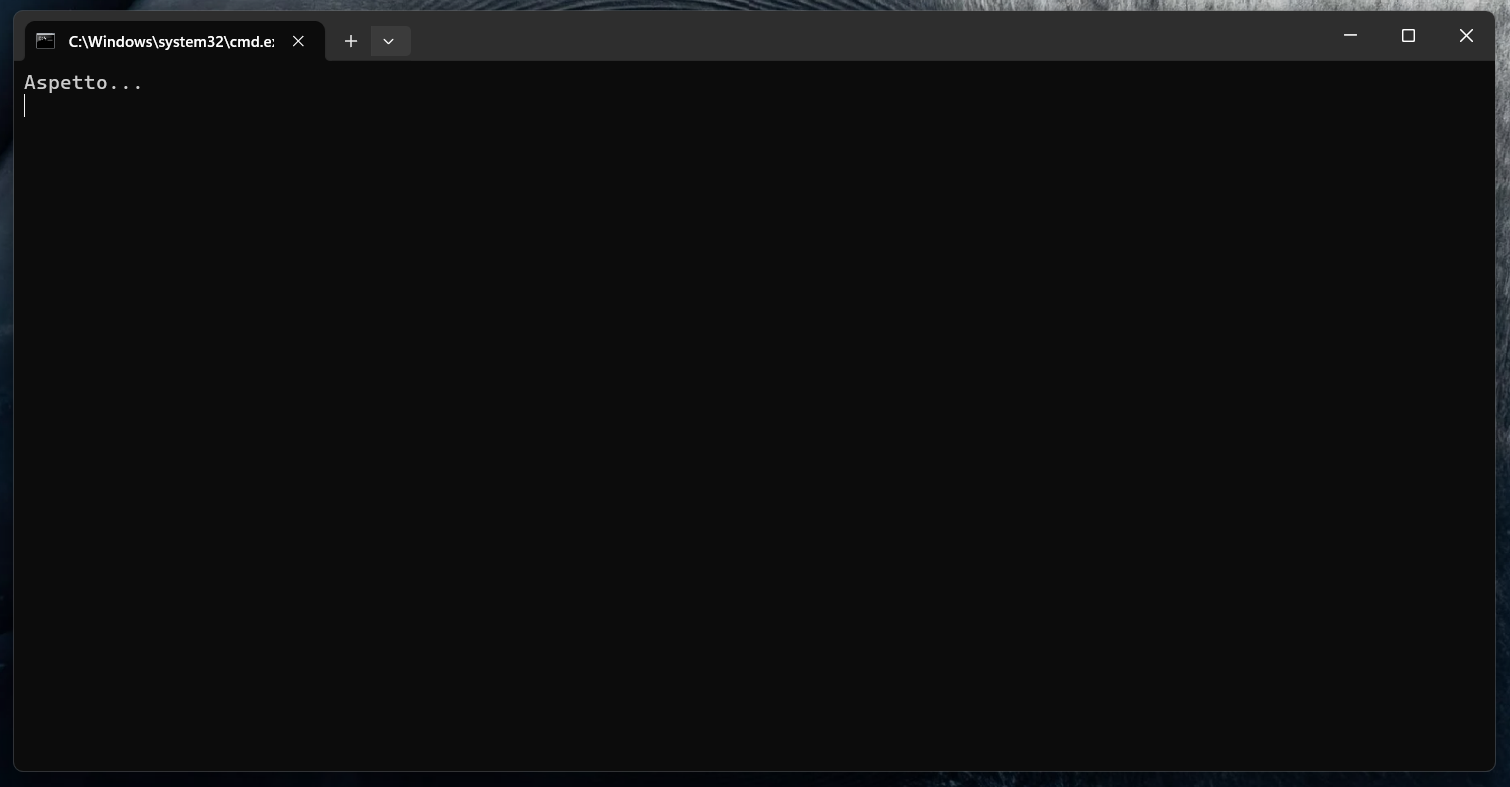
\includegraphics[width = 0.5 \textwidth]{images/normale funzionamento del server.png}
    \caption{Server in ascolto}
    
\end{figure}

\subsection{Esecuzione di QTB\_Client}

Per quanto riguarda il client, una volta avviato, mostrerà la seguente schermata.

\begin{figure}[h!]
    \centering
    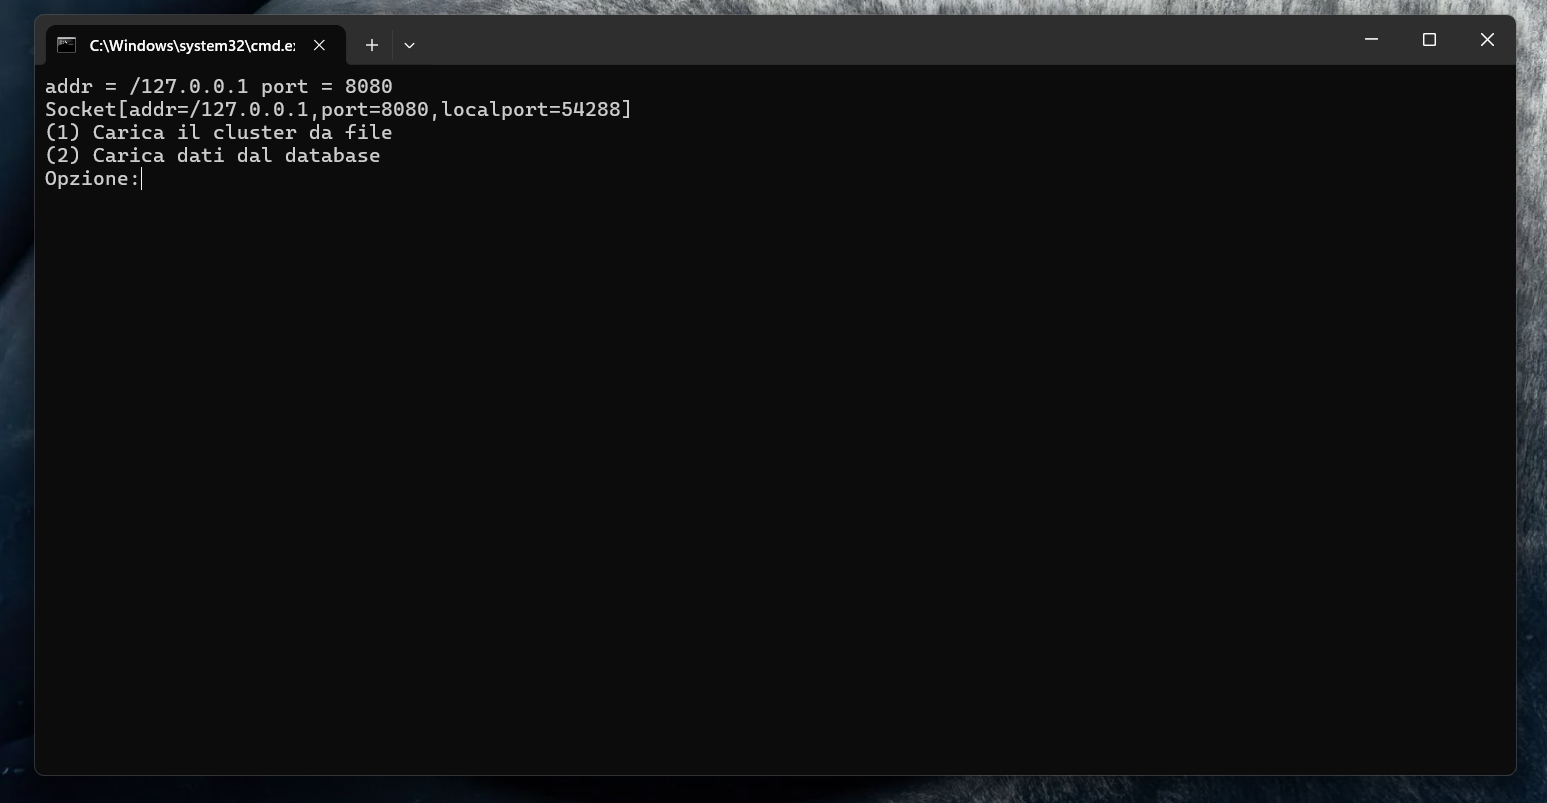
\includegraphics[width = 0.5 \textwidth]{images/normale funzionamento lcient.png}
    \caption{Schermata iniziale del client}
    
\end{figure}

\begin{tcolorbox}[  colback=white!5!white, colframe=gray, title={Avvertenza} ]

    Nel caso in cui il server non si sia avviato correttamente, o sia stato avviato il client prima del server, il client mostrerà la seguente schermata, che indicherà appunto che la connessione al server non è avvenuta correttamente.
    
    \begin{center} 
        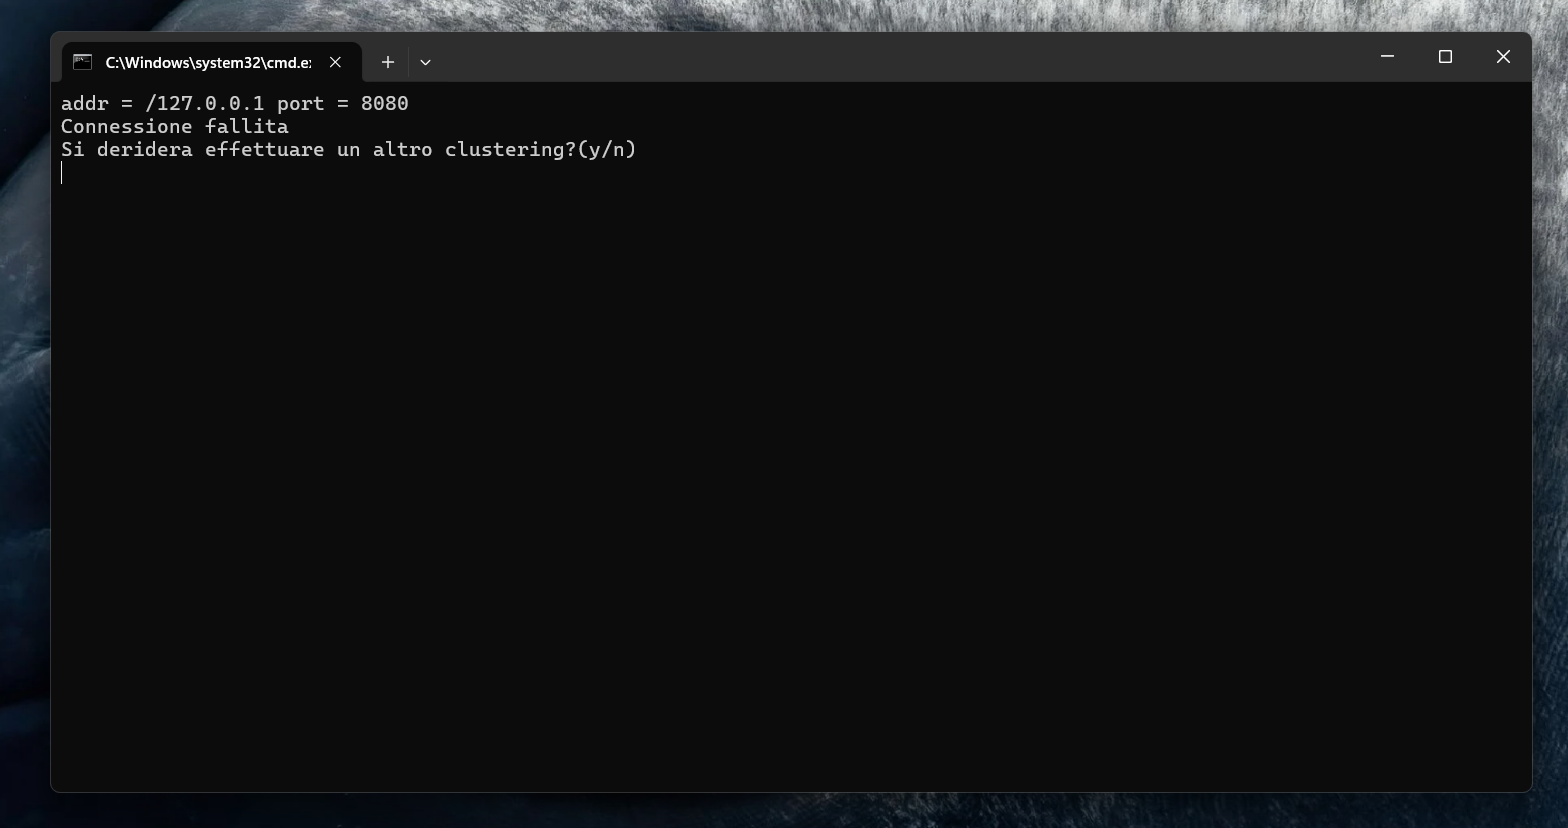
\includegraphics[width = 0.5 \textwidth]{images/connessione fallita.png}
    \end{center}
        
\end{tcolorbox}

Una volta assicurati che il client comunichi correttamente con il server, si potrà decidere se caricare i dati da un file di un clustering precedente o da un database.


Se si sceglie di caricare i dati da una tabella del database, si procederà con l'inserimento del nome della tabella da cui si vogliono estrarre i dati. Nel caso in cui tale tabella non sia presente nel database, il client avviserà l'utente con un messaggio di errore e chiedendo di inserire un nome valido. 

\begin{figure}[h!]
    \centering
    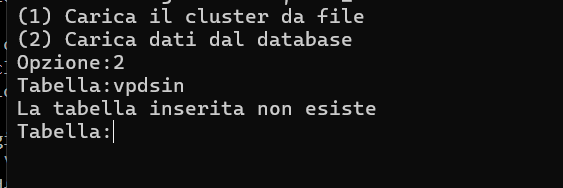
\includegraphics[width = 0.5 \textwidth]{images/teabella inesistente.png}
    \caption{Errore tabella non presente}
\end{figure}

Una volta scelto correttamente una tabella, si procederà nel determinare il raggio del clustering e, automaticamente, il programma restituirà il risultato. 

\begin{figure}[h!]
    \centering
    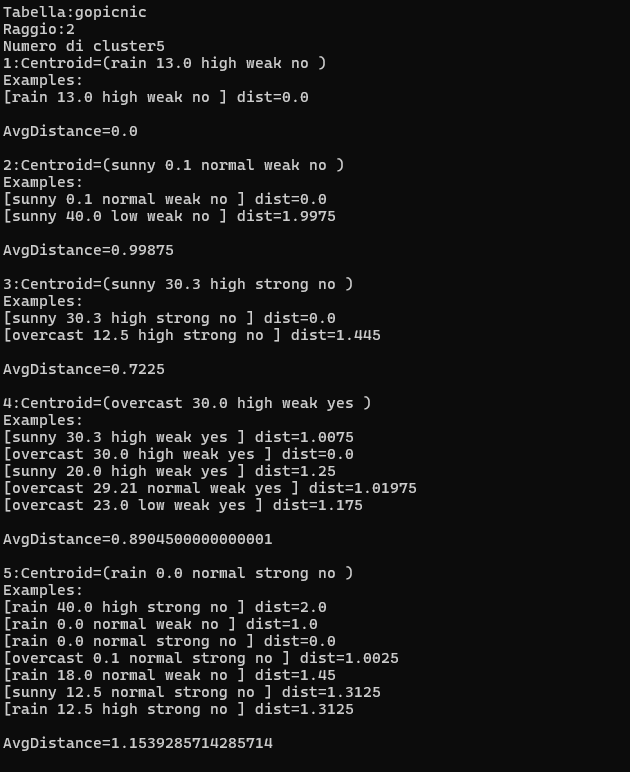
\includegraphics[width = 0.5 \textwidth]{images/risultato atteso.png}
    \caption{Risultato del clustering}
\end{figure}

\subsection{Test QT\_BASE}

Durante l'esecuzione del programma, può capitare che l'utente inserisca dei valori che quest'ultimo non è in grado di gestire. Chiaramente nonostante la presenza di queste situazioni, deve essere garantita la continuità di esecuzione del programma e la corretta amministrazione di queste situazioni estreme.

\subsection*{Gestione del raggio}

Nel caso in cui l'utente inserisca un valore del raggio maggiore del massimo raggio possibile, il programma restituirà un messaggio di errore e chiederà nuovamente il raggio.

Nel caso invece in cui l'utente inserisca un valore non numerico, il programma restituirà un messaggio di errore e chiederà nuovamente il raggio.

In entrambi i casi, il programma non si fermerà e continuerà a chiedere il raggio fino a quando non verrà inserito un valore corretto.

\begin{figure}[h!]
    \centering
    \subfloat[Valore del raggio troppo grande]{
        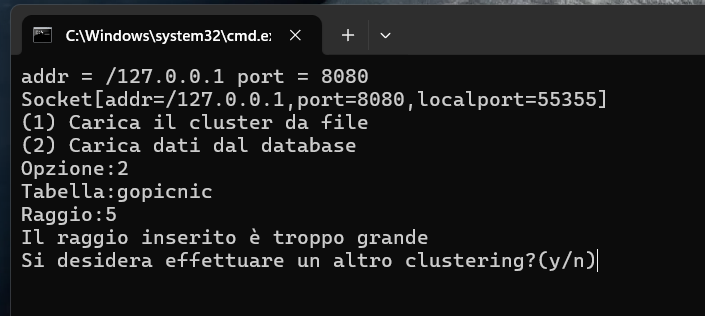
\includegraphics[width=0.45\textwidth]{images/troppo grande .png}
    }
    \hfill
    \subfloat[Valore del raggio non numerico]{
        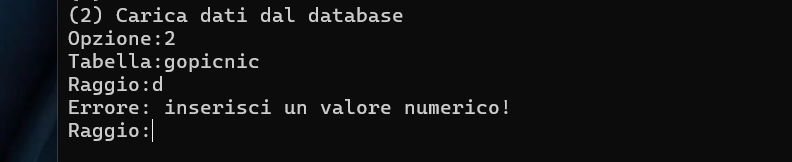
\includegraphics[width=0.45\textwidth]{images/valore non numerico .png}
    }
    \caption{Errori nel valore del raggio}
\end{figure}

\subsection*{Uscita dal programma}
Una volta calcolato il raggio, il programma chiederà all'utente se ha intenzione di effettuare nuovamente un clustering: in caso positivo chiederà nuovamente la misura del raggio, in caso opposto chiederà all'utente se vuole tornare al menù principale o chiudere il programma. 


\begin{figure}[h]
    \centering
    
\includegraphics[width = .5\textwidth]{images/richeista continuazione.png}
    \caption{Gestione finale clustering}
\end{figure}

Domandando all'utente se si vuole ritornare al menù principale, si gestisce la chiusura del programma e, allo stesso tempo, il ritorno al menù principale, ossia alla situazione iniziale. 

Inoltre, tale stratagemma previene lo spiacevole inconveniente per cui si è obbligati a forzare l'interruzione dell'esecuzione.

\end{document}